

The goal of the optimization system is to produce a solution to a user defined request.
When a user defines a request, as shown before, the arcs which connect those nodes are not defined, 
and thus, no solution can be produced.
After collecting the information regarding these arcs, it is possible to run 
an optimization algorithm which produces the best set of flights for the specific request,
according to some objective function.
However, depending on the specific request, the time necessary to collect 
the required flights, or the time necessary to produce a high quality solution may be very high,
due to high number of necessary flights, aswell as the computational complexity associated to this problem.

Because of the latency inherint to complex requests,
the optimization system will try to produce a random solution, whose overall quality is unknown,
in a very short time. This can usually be done using a single HTTP request,
because API's allow the aggregation of up to 9 flight queries,
and it enables the presentation of a very fast response,
reducing the latency felt by the user.
Furthermore, this type of random search corresponds to the currently available option 
for multicity flight searches. That is, every website which does multi city search, 
require the definition of a specific route and specific dates,
and it is this approach that will be taken to produce a first random solution.

Of course, the random solution produced is probably not the best,
because it is only one of the more than $N!$ possible solutions for a $N$ city multi trip request.
Thus, after producing the initial response, the optimization system  
will utilize more specialized algorithms to try to produce better solutions.
These algorithms usually require a complete cost matrix, 
and thus this process can only be undertaken after the Data Management System completed the construction 
of the family of necessary arcs.

Having the complete list of arcs, it is possible to run more complex optimization algorithms,
which are usually capable of producing better solutions, but which might take some time to do so.
A first simple heuristic algorithm that can be produced is the Nearest Neighbour,
which is probably capable of improving the quality of the previsouly defined random solution,
in a very short time.
On the other hand, two meta-heuristic algorithms, the Ant Colony Optimization and the Simmulated Annealing, 
will also be tested.
The objectives is to improve the quality of the solution as much as possible,
in a reasonable time. 

This process of solving the request using multiple optimization algorithm is illustrated in figure \ref{fig:optimization_system}.
Note that the \textit{Random} solution can be presented in a very short time, 
because it is not necessary to construct a complete multipartite graph, but simply a single random solution,
which can almost immediatly be presented to the user.
On the other hand, the \textit{N.N.} and \textit{Metaheuristic} solutions can only be produced 
after having a complete multipartite graph. Thus, it is expected that producing these solutions 
may take much more time compared to the random. 

\begin{figure}[htpb]
  \centering
  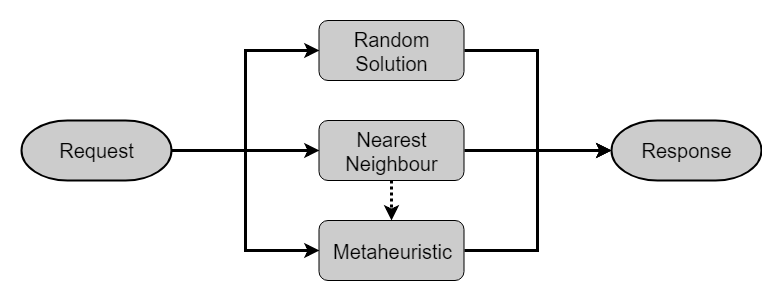
\includegraphics[width=\textwidth]{./Figures/system_design/utility.png}
  \caption{Simplified illustration of the optimization system, which utilizes different algorithms 
  to produce a solution to a user defined request.}
  \label{fig:optimization_system}  
\end{figure}

Having an optimization system which employes multiple, very different, optimization algorithms,
enables the comparison of both the time, and the quality of the proposed solutions.
We known apriori that the random solution is fast, and that its quality is probabily bad.
On the other hand, we expect the more specific algorithms to be slower, but present better solutions.
The goal than to verify if the solution is actually better, how significant the improvement is,
and how much time was necessary to produce such an improvement.

